上一节讨论的是在同一台机器上运行多个线程,而这些线程之间没有任何交互。如果能以一种方式将程序所做的工作分割到多个线程之间,那么无论如何都要这样做。

线程之间通常需要交互,因为它们正在为一个共同的结果工作。这种交互是通过线程之间,通过共享资源(内存)进行通信的方式进行。我们现在必须理解这对性能的影响。

假设我们要计算多个值的和,有很多数字要累加,但最后只有一个结果,所以想要在几个线程之间进行添加工作。因此线程在做加和时,结果值时必须进行交互。

\hspace*{\fill} \\ %插入空行
\noindent
\textbf{02\_sharing\_incr.C}
\begin{lstlisting}[style=styleCXX]
unsigned long x {0};
void BM_incr(benchmark::State& state) {
	for (auto _ : state) {
		benchmark::DoNotOptimize(++x);
	}
}
BENCHMARK(BM_incr)->Threads(2);
\end{lstlisting}

简单起见,这里将结果递增1(整数相加的代价与值无关,并且不想对不同值的生成进行基准测试,而只想对加法进行基准测试)。由于基准函数由每个线程完成,因此在这个函数中声明的任何变量都独立存在于每个线程的堆栈上,这些变量不共享。为了得到两个线程都参与的共同结果,变量必须在基准函数之外的文件范围内声明(这是个坏主意,但在微基准的非常有限的上下文中是必要和可接受的)。

当然,这个程序有一个比全局变量更大的问题:这是个错误的程序,其结果未定义。有两个线程递增相同的值,增加一个值需要3个步骤。程序从内存中读取值,在寄存器中增加值,然后将新值写回内存。两个线程完全可以同时读取相同的值(0),在每个处理器(1)上分别递增,然后写回。写第二个线程的线程只是重写第一个线程的结果,在两次增量之后,结果是1,而不是2。这是因为两个线程为了写入同一内存位置而进行了竞争,这种竞争称为\textbf{数据竞争}。

既然了解了为什么这种无保护的并发访问会出问题,那么最好忘记它。相反,请遵循这个一般的规则:如果在没有同步的情况下,让多个线程访问相同的内存位置,并且这些访问中有一个是写操作,结果是未定义的。这是非常重要的,没有必要确切地指出必须做哪些操作序列会得到不正确的结果。事实上,在这种推理过程中什么也得不到。当有两个或更多的线程访问同一个内存位置时,就会遇到数据竞争,除非能保证以下两件事中的一件:要么所有的访问都只读,要么所有的访问都使用了正确的内存同步(这一点我们还没有了解到)。

计算求和的问题要求将结果写入结果变量,所以访问肯定不是只读的。内存访问的同步通常由互斥锁提供,每次访问线程间共享的变量都必须由互斥锁保护(当然,所有线程的互斥锁必须相同)。

\hspace*{\fill} \\ %插入空行
\noindent
\textbf{03\_mutex\_incr.C}
\begin{lstlisting}[style=styleCXX]
unsigned long x {0};
std::mutex m;

{ // Concurrent access happens here
	std::lock_guard<std::mutex> guard(m);
	++x;
}
\end{lstlisting}

\texttt{lock\_guard}锁在其构造函数中锁定互斥锁,并在析构函数解锁。一次只有一个线程可以拥有锁,这样就可以对共享结果变量进行增加数值的操作。这时,其他线程被锁阻塞,直到第一个线程释放锁后才能获取锁。注意,只要有一个线程在修改变量,所有的访问(包括读和写)都必须阻塞。

锁是确保多线程程序正确性的最简单方法,但就性能而言,还挺难研究的。锁的实现相当复杂,会经常涉及系统调用。我们将从一个同步选项开始,在这个特定的例子中,这个方式会更容易分析:原子变量。

C++提供了一个将变量声明为原子变量的选项。这意味着对这个变量支持的所有操作都是不可中断的原子事务。任何观察这个变量的其他线程都将在原子操作前后看到它的状态,但绝不会在操作的中间看到它的状态。例如,C++中所有的整数原子变量都支持原子增量操作。如果线程正在执行这个操作,那么在第一个操作完成之前,其他线程都不能访问这个变量。这些操作需要一定的硬件支持,原子增量是一种特殊的硬件指令,它读取旧的值,增加它的值,然后写入新值,所有这些都作为一个单独的硬件操作。

我们的示例中,只需要一个原子自增。必须强调的是,无论使用什么同步机制,所有线程都必须使用相同的机制来并发访问特定的内存位置。如果在一个线程上使用原子操作,只要所有线程都使用原子操作,就不存在数据竞争。如果另一个线程使用互斥锁或非原子访问,那保护不起作用,结果依旧是未定义的。

用C++的原子操作重写基准测试:

\hspace*{\fill} \\ %插入空行
\noindent
\textbf{02\_sharing\_incr.C}
\begin{lstlisting}[style=styleCXX]
std::atomic<unsigned long> x(0);
void BM_shared(benchmark::State& state) {
	for (auto _ : state) {
		benchmark::DoNotOptimize(++x);
	}
}
\end{lstlisting}

程序现在是正确的,这里没有数据竞争。这并不一定准确,因为单个自增是在一个非常短的时间间隔内进行的,这里应该手动展开循环或使用宏,并在每次循环迭代中进行多次递增(已经在上一章中做了这一点,所以可以在那里看到这样的宏)。若线程之间没有交互,两个线程计算总和的时间将是一个线程计算总和的一半:

%\hspace*{\fill} \\ %插入空行
\begin{center}
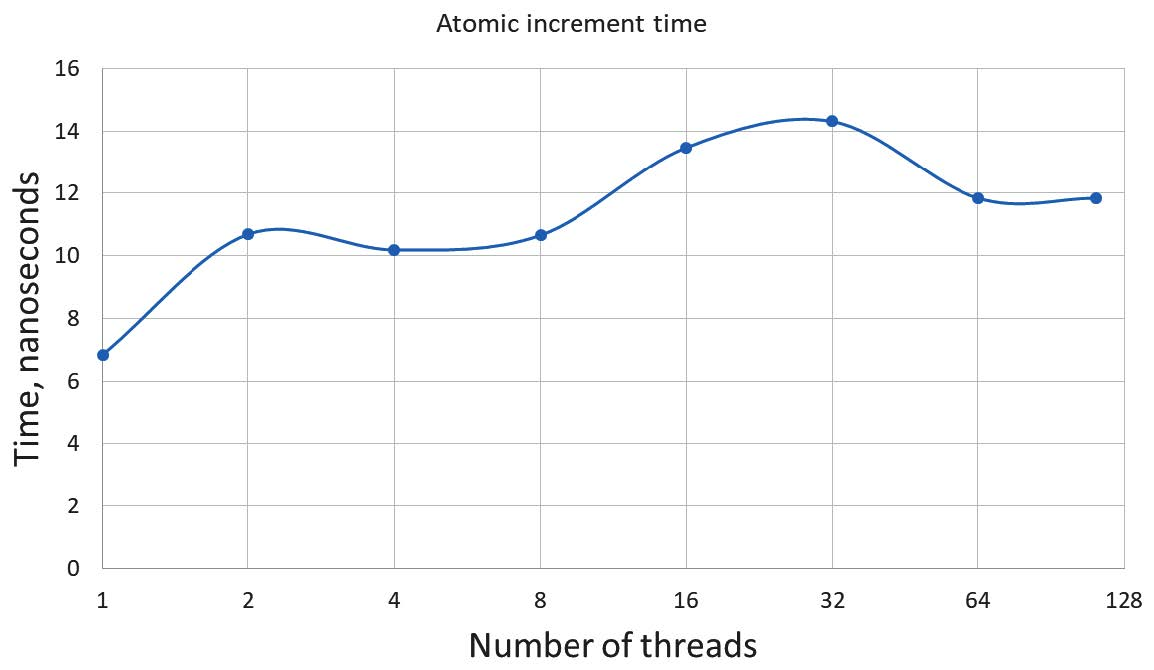
\includegraphics[width=0.9\textwidth]{content/1/chapter5/images/4.jpg}\\
图5.4 - 多线程程序中原子自增的时间
\end{center}

对结果进行了标准化,以显示单个增量的平均时间,即计算和除以相加总数的时间。这个程序的性能非常令人失望,不仅没有任何改进,在两个线程上计算总和要比在一个线程上花费更长的时间。

如果使用互斥锁,结果会更糟:

%\hspace*{\fill} \\ %插入空行
\begin{center}
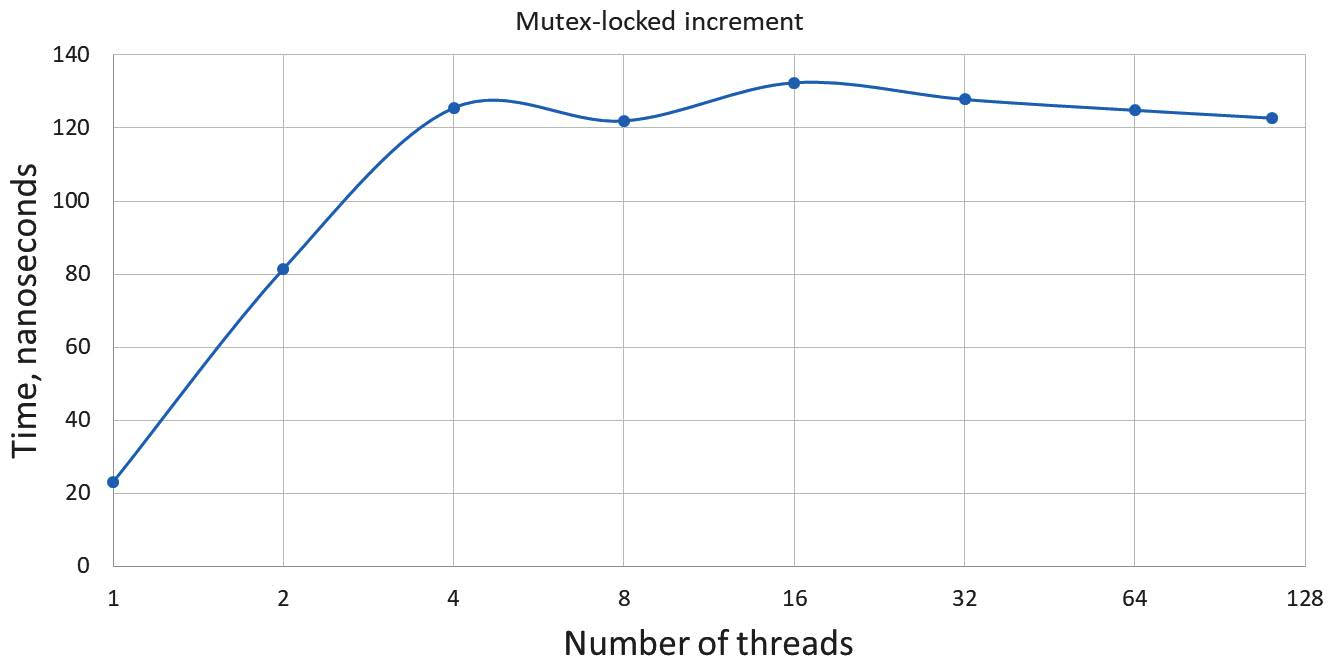
\includegraphics[width=0.9\textwidth]{content/1/chapter5/images/5.jpg}\\
图5.5 - 多线程程序中使用互斥量会增加耗时
\end{center}

首先,锁定互斥锁是一个相当耗时的操作,即使在一个线程上。互斥锁需要23纳秒,而原子变量需要7纳秒。随着线程数量的增加,性能会下降得更快。

可以从这些测试中了解到很多。程序中访问共享数据的部分永远不会扩展,访问共享数据的最佳性能是单线程性能。当有两个或更多的线程同时访问相同的数据,性能只会变得更糟。当然,如果两个线程在不同的时间访问相同的数据,它们不会交互,因此两次都获得了单线程性能。多线程的性能优势来自于线程独立计算,而不需要同步。这样的计算可以在不共享的数据上进行(无论如何,若希望程序结果正确),但是为什么对共享数据的并发访问有如此大的开销呢?下一节中,我们将了解其中原因,也将了解如何解析测试结果。








